\glsresetall
\chapter{Metodologia de Avaliação}
\label{chap.experiment-methodology}
Neste capítulo, será apresentado como a solução foi avaliada. Particularmente, as perguntas que guiaram o desenvolvimento dos experimentos para analisar a virtualização e a migração de processos no \nanvix foram:

\begin{enumerate}[start=1,label={Q\arabic*}]
    \item \label{item.q1}Qual impacto o isolamento da \uarea e do código e dados de usuário teve sobre o tempo de execução de operações do subsistema de \threads no \nanvix?
    \item \label{item.q2}Qual a eficiência da migração de processos no \nanvix de acordo com a quantidade de dados manipulados pela aplicação?
    \item \label{item.q3}Há sobrecarga no sistema de comunicação quando migramos aplicações paralelamente?
    \item \label{item.q4}O \daemon, em um mesmo \cluster, é capaz de atender requisições de migração variando o papel do \cluster na migração?
\end{enumerate}

Para responder a pergunta \ref{item.q1}, foi desenvolvido um experimento sobre a manipulação de \threads no \nanvix, que é o principal subsistema afetado pela \uarea. O experimento mensura os impactos na criação e junção de \threads através de diferentes perspectivas. Este experimento estressa o subsistema de threads através da criação e junção do máximo de \threads que o sistema suporta \ie 18 \threads. Especificamente, coletamos o tempo de execução, desvios e faltas ocorridas na \cache de dados e de instrução.

Para responder a pergunta \ref{item.q2}, foi desenvolvido outro experimento. O experimento mensura o tempo de transferência de um processo entre \clusters de acordo com os recursos utilizados \ie \threads e quantidade de páginas de memória alocadas dinamicamente. Neste teste, variamos a quantidade de páginas de memória alocadas dinamicamente entre 0 e 32; e \threads usadas pela aplicação entre 1 e 17. Dessa forma, nós avaliamos como ocorre a progressão do tempo de transferência de um processo desde a alocação mínima de recursos até a alocação máxima \ie desde 1 \thread e 0 páginas de memória até 17 \threads e 32 páginas de memória, em que cada página ocupa 4~KB.

Para responder a pergunta \ref{item.q3}, nós desenvolvemos um experimento que mensura o \downtime da aplicação quando variamos a quantidade de processos migrados paralelamente. Neste experimento são considerados quatro cenários de migração paralela em que cada processo é migrado uma vez entre um par de \clusters. Os cenários se diferenciam pela quantidade de processos e \clusters: 1, 2, 4 e 8 processos, o que abrange, respectivamente, 2, 4, 8 e 16 \cclusters. Um \iocluster é utilizado em todos os cenários com o intuito de registrar o tempo obtido.

Para responder a pergunta \ref{item.q4}, desenvolvemos um experimento que avalia a corretude do \daemon quando realizamos mais de uma migração envolvendo o mesmo \cluster e variando o papel deste na migração. Neste experimento, um processo é migrado de \cluster em \cluster até que percorra todos os \cclusters do processador \ie o processo é migrado realizando um movimento circular, passando do \cluster 0 para o 1, do 1 para o 2, e assim sucessivamente até retornar ao \cluster 0. O movimento circular garante que todos os \clusters façam duas migrações: uma como remetente e outra como destinatário, totalizando 16 migrações. 
% Destaca-se que quaisquer dois \clusters podem ser os envolvidos durante uma migração. O esquema de migração circular foi adotado porque conseguimos generalizar os \clusters envolvidos na migração, de modo que o processo \textit{cluster}$_n$ migrará para o \textit{cluster}$_{n + 1 \pmod{16}}$.

Todos os testes foram realizados no processador \mppa. Realizamos múltiplas replicações para garantir maior confiança estatística. Foram feitas 100 replicações para o primeiro experimento e 20 replicações para os demais. A medição de tempo no segundo e terceiro experimento foi feita utilizando a abstração de comunicação \sync.

Como as estruturas utilizadas por cada experimento variam, a quantidade de dados enviada também varia. Contudo, podemos generalizar a quantidade de \bytes enviada através da Equação \ref{eq.1}. Na Equação \ref{eq.1} o identificador \texttt{U} representa o tamanho do binário de usuário, \texttt{UA} o tamanho da \uarea, \texttt{SYSB} o tamanho da tabela de gerenciamento das chamadas de sistema, \texttt{PGDIR} o tamanho da tabela de diretórios de páginas, \texttt{PGTAB} o tamanho da tabela de página, \texttt{KSIDS} o tamanho da lista de gerenciamento de páginas de \kernel, \texttt{KSPHYS} a soma do tamanho das páginas de \kernel em uso, \texttt{FBMP} o tamanho do \bitmap de gerenciamento dos \frames e \texttt{FPHYS} a soma do tamanho dos \frames usados pela alocação dinâmica de páginas de memória. A soma de todas essas variáveis resulta na quantidade de dados manipulados (\texttt{DM}) em \bytes.

\begin{equation}\label{eq.1}
    DM = U + UA + SYSB + PGDIR + PGTAB + KSIDS + KSPHYS + FBMP + FPHYS
\end{equation}

Algumas dessas variáveis são constantes nos experimentos. Substituindo-as pelos seus respectivos valores em \bytes obtemos a Equação \ref{eq.2}.

\begin{gather}
    DM = 10608 + 2112 + 1920 + 4096 + 4096 + 160 + KSPHYS + 16 + FPHYS\\
    DM = 23008 + KSPHYS + FPHYS\label{eq.2}
\end{gather}

Sendo assim, percebemos que a quantidade de dados enviada varia em função da quantidade de páginas de \kernel em uso e da quantidade de páginas alocadas dinamicamente. Tendo em vista que as variáveis do experimento são a quantidade de \threads e a quantidade de páginas alocadas dinamicamente, é importante entender como essas variáveis impactam em \texttt{KSPHYS} e \texttt{FPHYS}. Primeiro, o \texttt{KSPHYS} muda quando uma thread é criada. Nesta operação, duas páginas de \kernel são alocadas para esta nova \thread: uma para a pilha de execução em espaço de usuário; e outra para a pilha de execução em espaço de \kernel. Segundo, o \texttt{FPHYS} muda quando página de usuário é dinamicamente criada. Quando isso acontece, aumentamos o espaço do usuário em mais uma página \ie aumentamos o \texttt{FPHYS} em uma página (4096~B). Além disso, quando alocamos a primeira página de usuário, uma página de \kernel é utilizada como tabela de páginas para essa e as possíveis novas páginas a serem alocadas. Arranjando esses dados na Equação \ref{eq.2}, obtemos:

\[
    DM = 
\begin{cases}
    23008 + 4096(2 \times NTHREADS),& \text{se } NPAGES= 0\\
    23008 + 4096(2 \times NTHREADS + NPAGES + 1),& \text{se } NPAGES > 0
\end{cases}
\]
ou simplesmente:
\begin{equation}\label{eq.3}
    DM = 23008 + 4096(2 \times NTHREADS + NPAGES + min(NPAGES, 1))
\end{equation}

Onde \texttt{NTHREADS} é a quantidade de \threads criadas e \texttt{NPAGES} a quantidade de páginas criadas.


Quanto ao funcionamento dos experimentos, no início do teste todos os \clusters sincronizavam entre si através do \sync. Neste momento, o \iocluster iniciava uma contagem de ciclos. Ao final do experimento, todos os \clusters envolvidos sincronizavam novamente. Neste momento, o \iocluster parava a contagem de ciclos e esse era o tempo que a migração demorou até seu término. Destaca-se que nos experimentos que precisavam de algum \setup inicial, o tempo de \setup não foi considerado. Por exemplo, no segundo experimento, o tempo para a criação de \threads, alocação e manipulação das páginas dinamicamente alocadas não é contabilizado no tempo final. O resultado, portanto, engloba apenas o \downtime da aplicação.



\chapter{Resultados Experimentais}
\label{chap.results}

Neste capítulo, serão apresentados os resultados obtidos através dos experimentos desenvolvidos.
% A solução foi avaliada em etapas anteriores ao desenvolvimento atual do trabalho e os resultados seguintes englobam apenas o subsistema de \threads do \nanvix. 
% \todo{Seria bom colocar um capítulo de metodologia com perguntas que gostariamos de responder e detalhamento dos experimentos}
% %
% Para avaliar o impacto das mudanças feitas para a virtualização, foram desenvolvidos experimentos sobre a manipulação de \threads e suporte à migração de processos no \nanvix. Todos os experimentos foram executados no processador \mppa e os resultados mostrados são valores médios de 100 replicações de cada experimento para garantir 95\% de confiança estatística, resultando em um desvio padrão inferior a 1\%.
\begin{figure}[tb]
	\centering
    \caption{Impactos da virtualização sobre a manipulação de \threads.
    \label{fig.threads}}%
	\subcaptionminipage[fig.fork-join]%
                   {.55\textwidth}
                   {Tempo de criação de \threads.}
                   {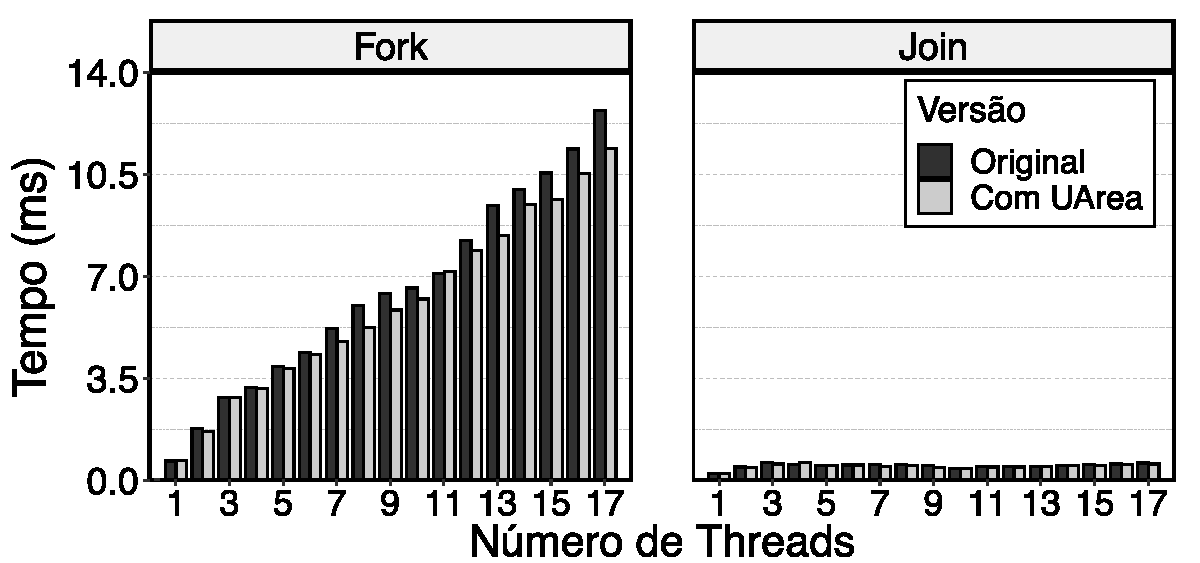
\includegraphics[width=\textwidth]{content/images/fork-join-kernel-time-bars.pdf}}
	\quad
	\subcaptionminipage[fig.kernel-counters]
                   {.4\textwidth}
                   {Métricas do \kernel.}
                   {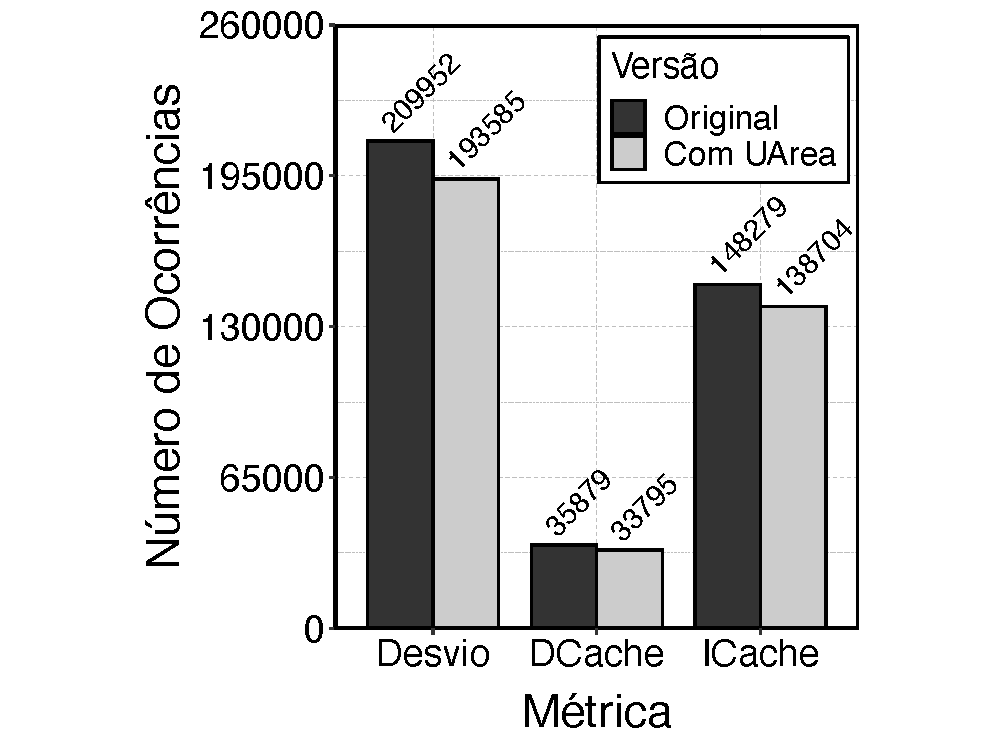
\includegraphics[width=\textwidth]{content/images/fork-join-kernel-counters.pdf}}
    \fonte{Desenvolvido pelo autor.}
\end{figure}

\begin{figure}[tb]
    \centering
    \caption{\Downtime da aplicação durante o experimento de migração fixando a quantidade de páginas alocadas dinamicamente}
    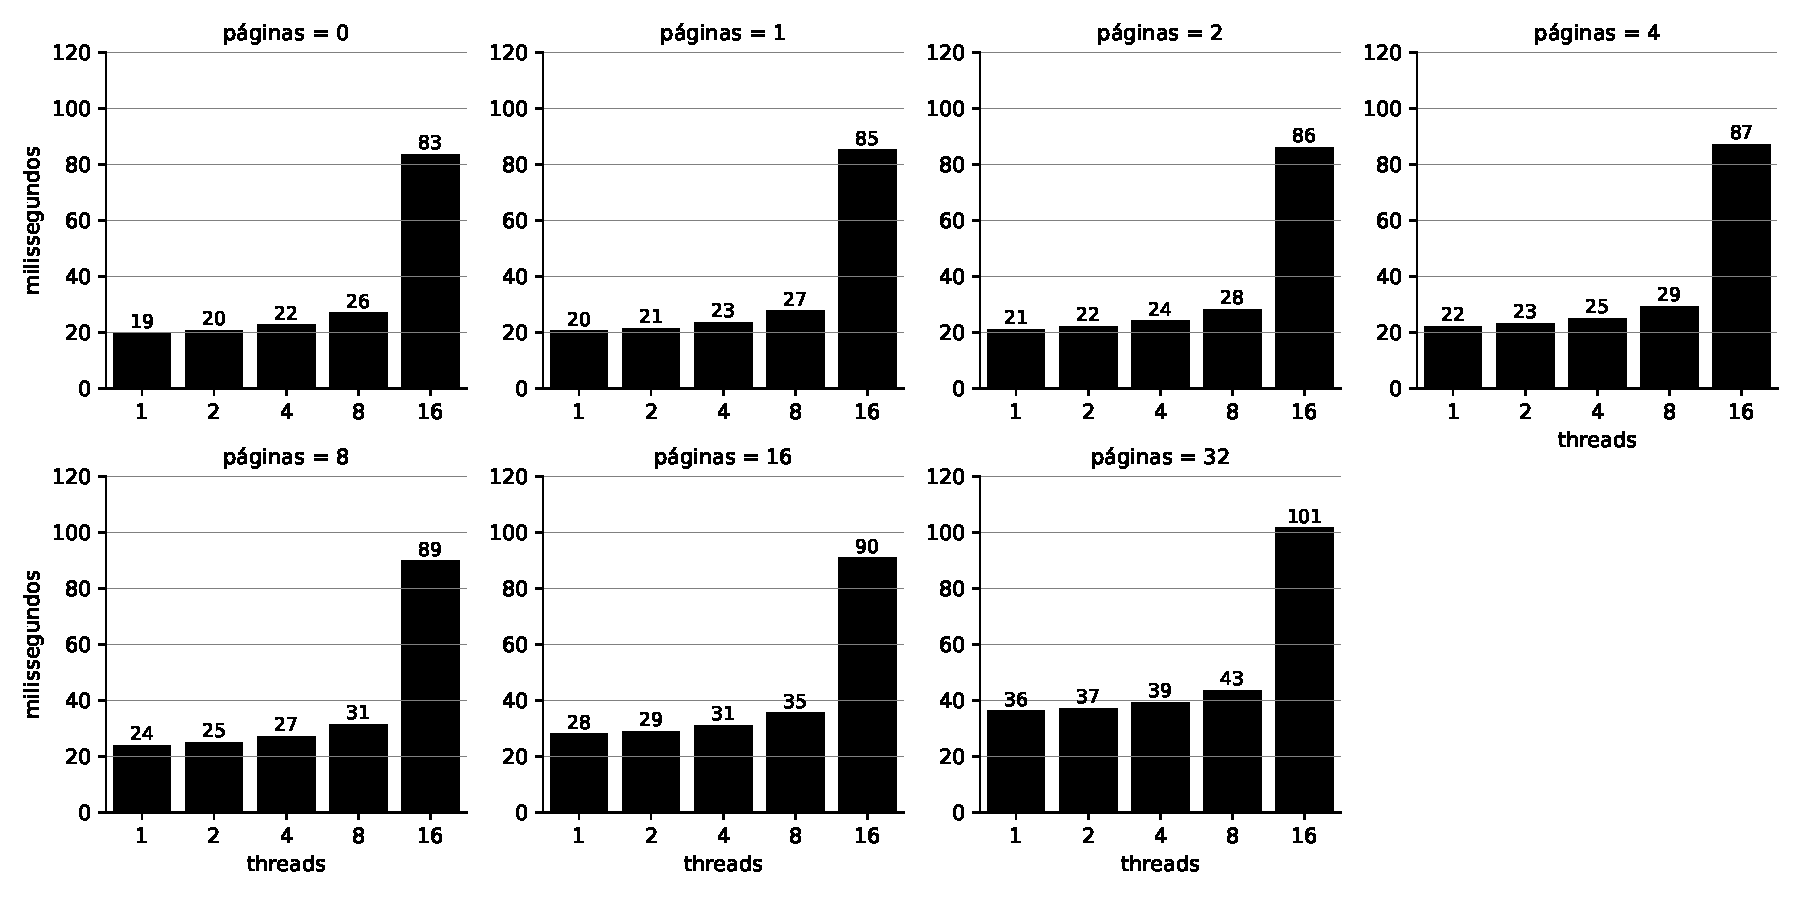
\includegraphics[width=\linewidth]{content/images/multiple_threads_pages.pdf}
    \label{fig.mtpages}
    \fonte{Desenvolvido pelo autor.}
\end{figure}

\begin{figure}[tb]
    \centering
    \caption{\Downtime da aplicação durante o experimento de migração fixando a quantidade de \threads}
    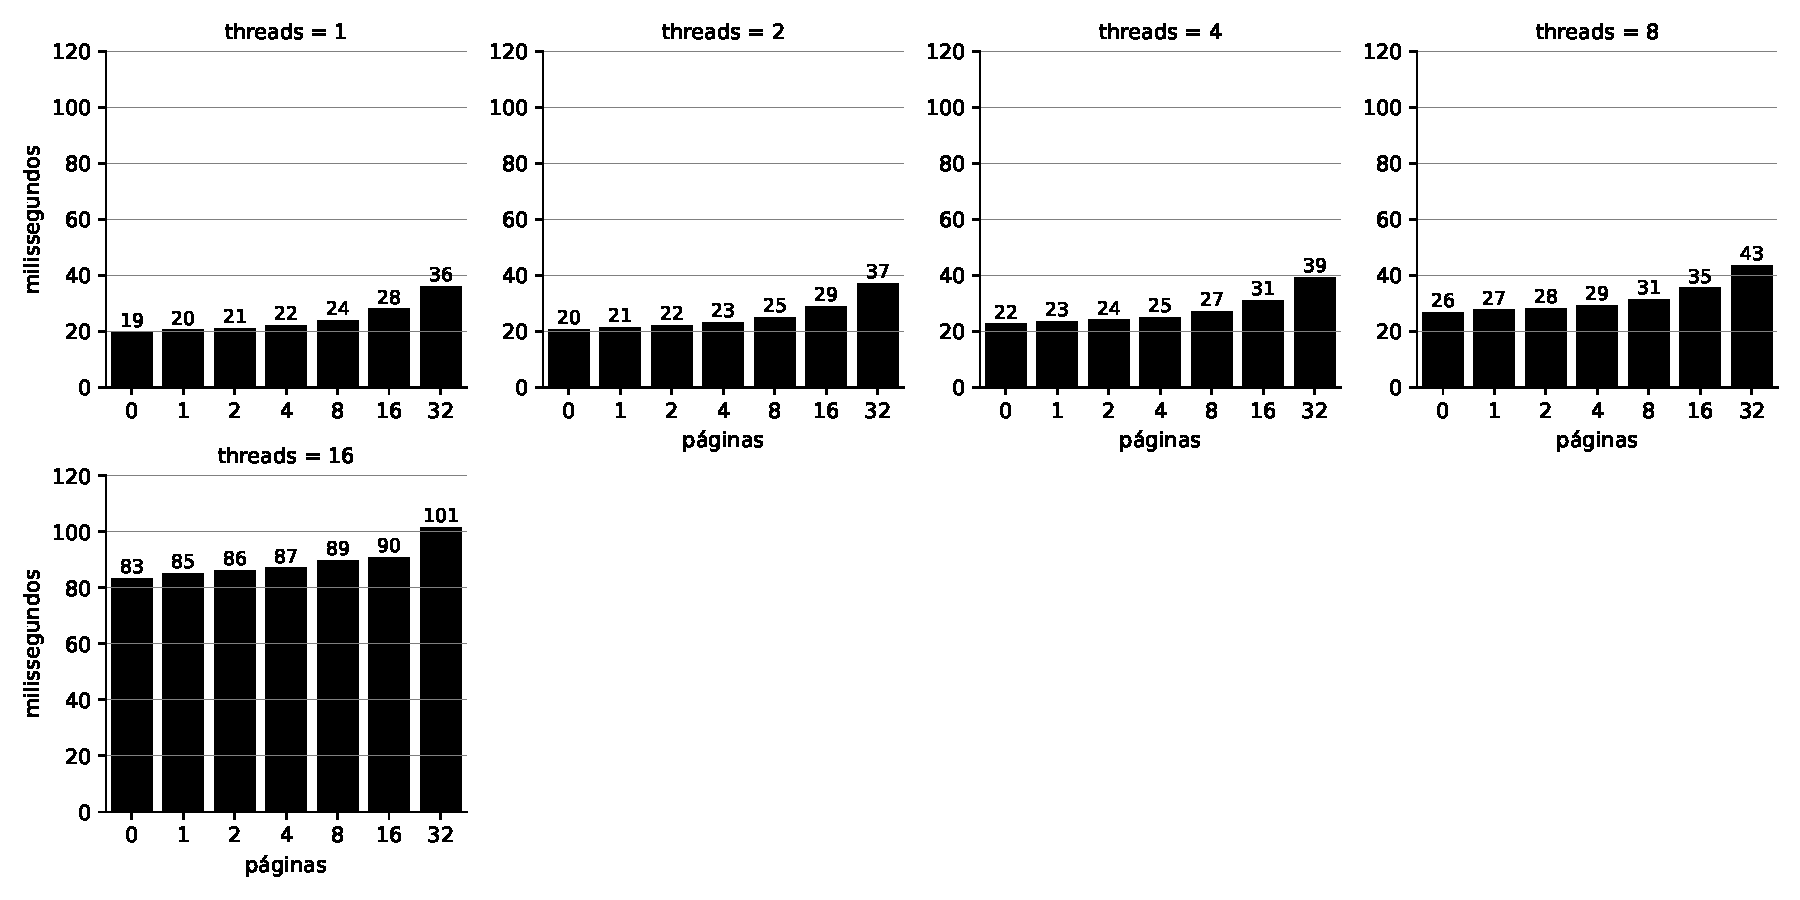
\includegraphics[width=\linewidth]{content/images/multiple_threads_threads.pdf}
    \label{fig.mtthreads}
    \fonte{Desenvolvido pelo autor.}
\end{figure}

\section{Análise do Impacto da UAREA e do Isolamento de Código e Dados de Usuário sobre a Manipulação de \threads}

Ao analisar o isolamento da aplicação através da UArea e separação do binário de usuário e kernel, percebemos um impacto positivo no subsistema de threads do Nanvix. A \autoref{fig.fork-join} ilustra que o \nanvix obteve um leve ganho de desempenho na operação de criação de \threads e não introduziu mudanças significativas na operação de junção de \threads. A \autoref{fig.kernel-counters} mostra a origem do aumento da performance na operação de criação de \threads, exibindo a quantidade de desvios e faltas nas \caches de dados e instrução. Percebemos que houve uma diminuição de:
\begin{inlinelist}
    \item 7,8~\% na quantidade de desvios;
    \item 5,8~\% na quantidade de faltas na \dcache; e
    \item 6,45~\% na quantidade de faltas na \icache.
\end{inlinelist}
Isso ocorre porque a \uarea explora melhor a localidade espacial dos dados, já que os dados estão aglomerados em um espaço menor da memória. Como consequência disso, o número de faltas na \cache e de desvios diminui, resultando em um aumento de desempenho.

\section{Análise do \downtime da Migração de Acordo com a Quantidade de Dados Manipulados}

A \autoref{fig.mtpages} e a \autoref{fig.mtthreads} mostram a progressão de tempo sobre diferentes perspectivas (fixando-se as páginas e \threads, respectivamente). Como o esperado, o \downtime aumenta quanto maior for o número de páginas e \threads, com um mínimo de 5,26~\% e uma máximo de 431~\%. Ou seja, quanto maior for a memória utilizada, maior o tempo de comunicação entre os \clusters. Além disso, a quantidade de \threads se destaca por apresentar maior expressividade no tempo contabilizado em comparação com a quantidade de páginas. Isso acontece porque uma \thread requer mais dados migrados além de uma página \eg é preciso migrar duas pilhas de execução, que totalizam duas páginas de memória e as estruturas de manipulação dessa \thread.

De maneira geral, o \downtime é aproximadamente descrito pela Função \ref{eq.downtime}:

\begin{equation}\label{eq.downtime}
    \begin{split}
        f(p, t) = \frac{17}{32} \times p+t+18
    \end{split}
\end{equation}

A Função~\ref{eq.downtime} aproxima a progressão de tempo até 15 \threads. Contudo, como podemos observar nas Figuras \ref{fig.mtpages} e \ref{fig.mtthreads}, ocorre uma disparidade com 16 \threads, afetando a natureza linear observada até 15 \threads. Isso acontece porque o \mppa possui 16 núcleos em um \cluster e, como o \nanvix apresenta um \microkernel assimétrico, um núcleo é reservado exclusivamente para a execução de \threads e tarefas do sistema. Desta forma, ao criar 16 \threads, nós extrapolamos a quantidade de núcleos disponíveis ao usuário. A competição de recursos entre duas \threads introduz, em média, 230~\% de sobrecarga ao \downtime, variando entre 198~\% e 246~\%. Ou seja, o salto numérico observado nas Figuras \ref{fig.mtpages} e \ref{fig.mtthreads} é resultado do tempo extra utilizado no experimento para o gerenciamento das \threads, já que temos mais \threads do que núcleos em que estas podem executar.


\section{Análise do Impacto de Migrações Paralelas sobre o Sistema de Comunicação}

Como ilustrado pela \autoref{fig.parallel}, o experimento que mensurava o \downtime da aplicação quando múltiplas migrações aconteciam simultaneamente, mostrou que a quantidade de migrações paralelas não impacta significativamente o tempo. Destaca-se que nesse experimento foram migradas aplicações que usavam o máximo de recursos de sistema. Mesmo assim, a quantidade de dados não foi suficiente para impactar no \downtime, o que significa que a topologia e a taxa de transferência da \noc do \mppa supre a demanda de transferência de dados. Considerando os cenários em que há 1, 2, 4 ou 8 migrações simultâneas, o \downtime médio foi em torno de 113~ms.


\begin{figure}[ht!]
    \centering
    \caption{\Downtime da aplicação em função da quantidade de migrações paralelas}
    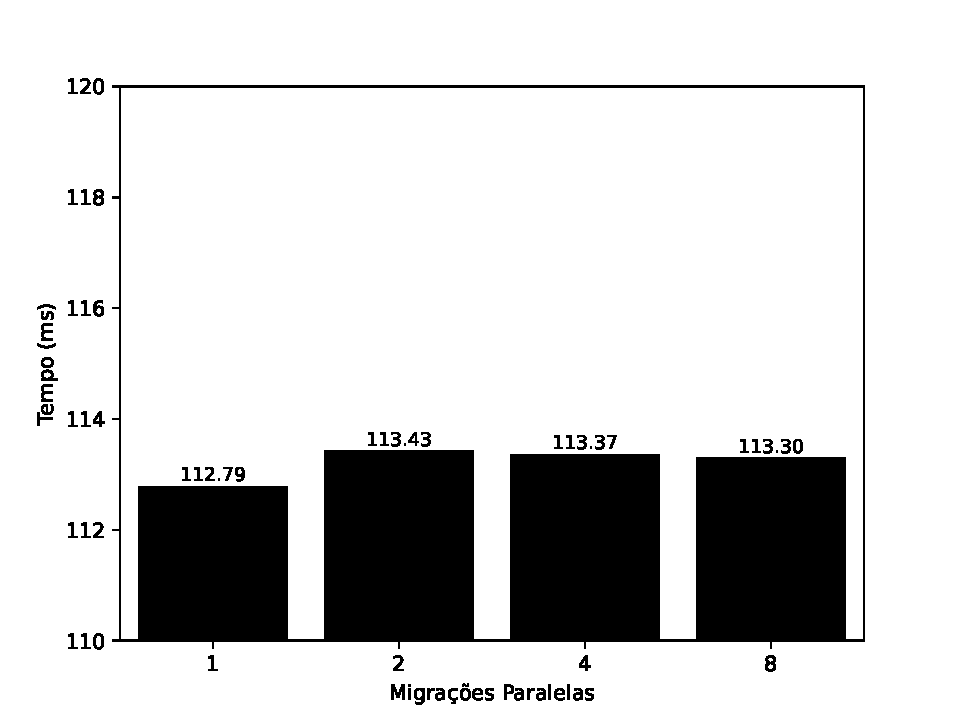
\includegraphics[width=0.7\linewidth]{content/images/parallel.pdf}
    \label{fig.parallel}
    \fonte{Desenvolvido pelo autor.}
\end{figure}

\section{Análise da Capacidade do \daemon Realizar Múltiplas Migrações Utilizando um mesmo \cluster}

O teste que visava a comprovação da consistência e corretude do \daemon executou completamente sem ocorrência de erros. Isso significa que:
\begin{inlinelist}
    \item o \daemon é capaz de ser reusado no mesmo \cluster diversas vezes independentemente do papel do \cluster na migração; e
    \item é possível um processo ser migrado diversas vezes para diferentes \clusters, até mesmo em movimento circular envolvendo todos os \clusters
\end{inlinelist}.

Esse comportamento é possível porque o \daemon é totalmente separado da aplicação e está associado ao \kernel. Isso porque está contido nas seções de \kernel do binário e sua execução é sustentada por \tasks, que são executadas por uma \thread de sistema, e não de usuário. Dessa forma, é possível que o \daemon conclua a migração como receptor e, logo em seguida, a partir da requisição da aplicação que acordou, volte a migrar.